\documentclass[11pt,a4paper]{article}
\usepackage[T1]{fontenc}
\usepackage[utf8]{inputenc}
\usepackage{lmodern}
\usepackage[margin=24mm]{geometry}
\usepackage{amsmath,amssymb,booktabs,array,graphicx,xcolor,microtype}
\usepackage{xurl}
\usepackage[colorlinks=true,linkcolor=blue!45!black,citecolor=blue!45!black,urlcolor=blue!45!black,breaklinks=true]{hyperref}
\emergencystretch=2em
\setlength{\parskip}{4pt}
\setlength{\parindent}{0pt}
\newcommand{\doctype}{Preprint}
\newcommand{\docversion}{v1.0}
\newcommand{\docdate}{31 October 2026}
\newcommand{\versiondoi}{10.5281/zenodo.23851369}
\newcommand{\conceptdoi}{10.5281/zenodo.23851368}
\newcommand{\docrepo}{github.com/fsantibanezleal/CAOS\_OreBridge}
\newcommand{\headerblock}{\begin{center}\fbox{\parbox{0.94\textwidth}{\small\raggedright
\textbf{\doctype}\quad$\cdot$\quad\docversion, \docdate\quad$\cdot$\quad Licence CC BY 4.0\\[2pt]
CAOS open-research programme\quad$\cdot$\quad OreBridge\\[2pt]
Version DOI: \href{https://doi.org/\versiondoi}{\texttt{\versiondoi}}\\
Concept DOI (always latest): \href{https://doi.org/\conceptdoi}{\texttt{\conceptdoi}}\\[2pt]
Not peer reviewed. Source code, data and computational results:\\
\href{https://github.com/fsantibanezleal/CAOS_OreBridge}{\texttt{\docrepo}}
}}\end{center}\vspace{4pt}}
\title{Transport-aligned robust reconciliation can degrade discrepancy localization: a controlled plant-network study}
\author{Felipe Santibáñez-Leal\\\small CAOS open-research programme, Santiago, Chile\\\small ORCID: 0000-0002-0150-3246}
\date{}
\begin{document}
\maketitle
\headerblock
\begin{abstract}
Conservation and model compatibility can produce coherent estimates without identifying which observation caused a discrepancy. A controlled sixteen-channel plant network compares weighted and Huber reconciliation, engineering thresholds, a trained causal histogram predictor and transport-aligned robust fusion with a fixed dry-solids relation. Twelve fault/control families, sixteen held-out seeds and four severity slots yield 6144 method/scenario cells. TASC recall is 0.3419063, compared with 0.3362188 for aligned Huber, 0.8399375 for the causal predictor and 0.5190938 after removing topology. The paired recall difference from no-topology is -0.1771875 with 95 percent seed-block interval [-0.1792188,-0.1752812]. Complete-frame methods also withhold more numerical entries, so coverage and source-valid comparisons accompany pooled ratios. Independent null-space optimization reproduces 48 robust objectives within numerical tolerance. The results distinguish optimization correctness, causal evidence timing and fault identifiability. They refute a general superiority claim for this particular equality/prior combination on the authored process, without showing that physical conservation is generally unhelpful or establishing operating-plant performance.
\end{abstract}

\section{Introduction}
A process balance can reveal incompatible measurements while leaving the cause ambiguous. Three noisy flow readings may not satisfy one conservation equation; weighted reconciliation supplies a unique statistical adjustment under an assumed covariance. That uniqueness comes from the model and does not certify which instrument, process relation or time assumption was wrong. The distinction becomes consequential when a residual is mapped to a colored equipment symbol.

Mineral-processing data reconciliation already combines measurements and physical constraints~\cite{sadeghi}. Robust losses limit large standardized deviations~\cite{huber}. Learned multivariate detectors can instead use recurring temporal relationships, including graph-based forecasting~\cite{gdn}. These approaches encode different information and need a common evaluation that retains both missed disturbances and false alerts. A physically plausible result is not, by itself, evidence of better localization.

The question is whether causal parcel alignment, Huber projection and an uncertain reference relation improve a specific controlled detector together. The transport-aware formulation is called Topology-Aware State Coherence (TASC). Its current prior is a fixed dry-solids ratio driven by observed upstream feed. It is not a new fundamental robust estimator, a complete industrial twin or a fusion of every source displayed by the associated plant interface. The combination is tested through timing, prior and topology removal.

The experiment is deliberately synthetic and short. Its value is the ability to inspect causal support, null-space ambiguity, known input rejection and paired failure cases. A negative result is substantial: removing topology improves recall and precision. This motivates examining how an equality projection spreads innovations, while separating that finding from a claim about all conservation-based estimators.

\section{Related work and task definition}
\subsection{Reconciliation and robust residuals}
Weighted constrained least squares chooses the nearest admissible state under a covariance model. Huber reconciliation replaces a globally quadratic penalty with one that grows linearly for large standardized residuals. Mineralogical constraints can add information beyond bulk balances~\cite{sadeghi}; the present network uses only eleven homogeneous bulk solids/water factors. Its numerical implementation is not a replication of that publication's complete mineralogical formulation.

The target here is pointwise discrepancy detection and localization under stated labels. A changed recovery relation is a modeled process change with affected coordinates, whereas a changed healthy transport delay is a no-sensor-fault control. Those choices define the task and should not be mistaken for universal operational alarm truth. A transport change may be worth investigating even when counted as a false fault alert in this experiment.

\subsection{Temporal learning and missing observations}
GDN learns sensor relationships for multivariate anomaly detection~\cite{gdn}. GST-Pro addresses missing values and irregular multivariate observations~\cite{gstpro}. They are related work and not implemented comparators. The actual learned alternative is maintained histogram gradient boosting~\cite{hgb}, fitted per channel using four complete earlier multichannel vectors. This representative model supplies a real temporal comparison without a global best-detector claim.

Known quality masks emulate acceptance by an ingestion contract. They are provided to the numerical preparation and are not discovered by a learned quality detector. Rejected finite values must be excluded before lag construction, not merely removed from the final target confusion count. Otherwise a misunit or misbound value can alter predictions of valid neighboring channels. Last accepted input is carried only inside the predictor, with explicit nominal initialization.

\section{Controlled process and causal support}
\subsection{Channels and conservation factors}
Sixteen channels represent dry-solids or water rates on one authored reference network. Dry-solids nominal flow starts at 720\,t/h, reaches a combined grinding-circuit reference of 2520\,t/h with 1800\,t/h recycle, and separates approximately 18.5991\,t/h concentrate and 701.4009\,t/h tailings. Four water channels describe make-up, return, tank inflow and outflow. Water and solids never enter the same factor row.

Let $\mu$ denote positive nominal flows, $d_i$ the channel delays and $L(t)$ an authored seeded source-load history. Clean observations satisfy a delayed relation approximately of the form
\begin{equation}
 x_i^{true}(t)=\mu_i L(t-d_i),\qquad
 y_i(t)=x_i^{true}(t)+\epsilon_i(t),
\end{equation}
with independent reference sensor noise at $\sigma_i=\max(0.01\mu_i,0.1)$. Eleven fixed conservation rows form $A$. The clean aligned process obeys $Ax=0$ by construction. This is an algebraic control, not independent evidence that the assumed delays describe a real plant.

\subsection{Alignment and availability time}
With $D=\max_i d_i=14$\,s, causal alignment is
\begin{equation}
 y_i^{aligned}(t)=y_i(t-(D-d_i)).
\end{equation}
Only present or earlier observations contribute. The first fourteen rows are unavailable. At availability time $t$, channels can describe different earlier wall-clock readings belonging to the same modeled parcel. A score must remain associated with its actual evidence time. Assigning an aligned score to a raw value at the same array index would silently change its interpretation.

Each exported method has a per-channel evidence-lag vector. Aligned methods use $D-d_i$ and simultaneous methods zero. Both numerical truth and source validity receive the same alignment for comparison. A physical change in the recovery or delay family updates current synthetic process truth; an old reference trajectory is not mislabeled as the current state.

\begin{figure}[htbp]\centering
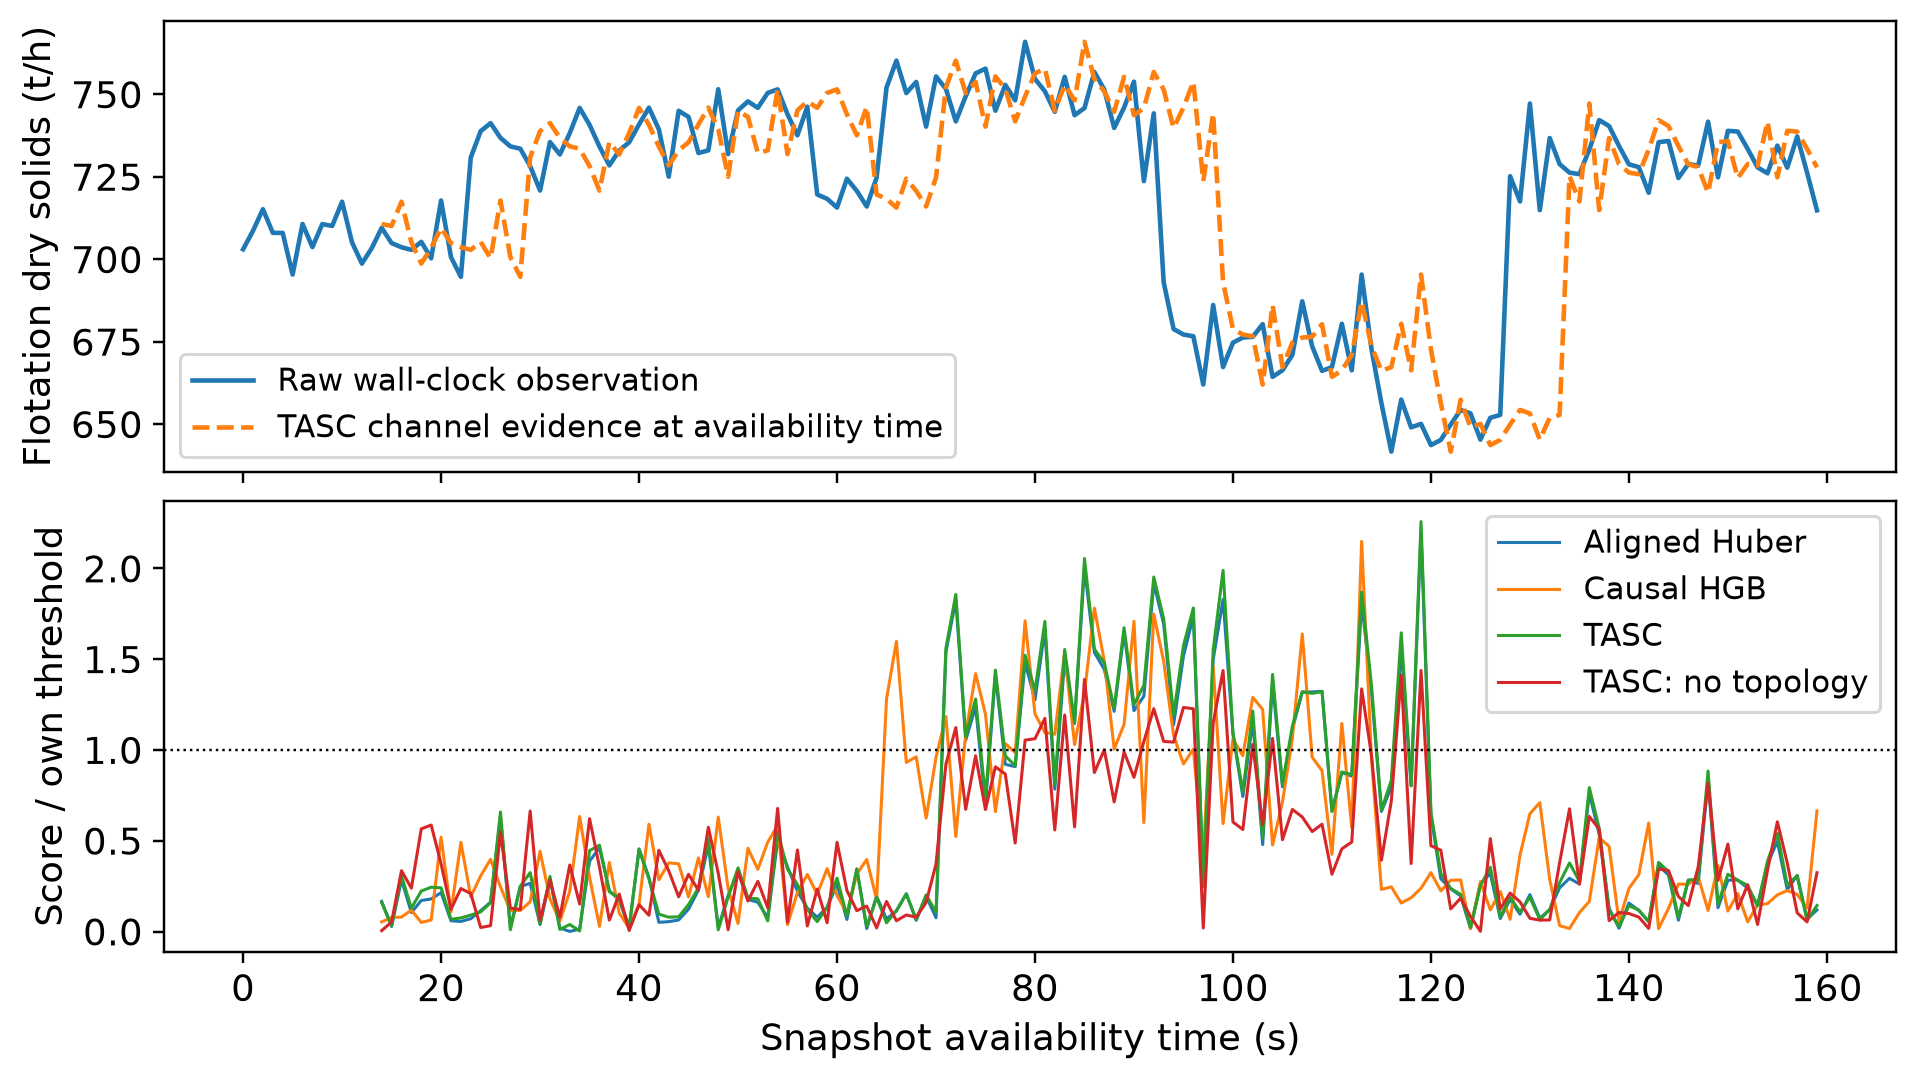
\includegraphics[width=.96\textwidth]{../shared/evidence-time.png}
\caption{An actual held-out feed-bias example. Aligned method scores refer to the earlier evidence shown at availability time. Common normalized boundaries do not imply equivalent losses or information sources.}
\end{figure}

\section{Methods and mechanism tests}
\subsection{Threshold, WLS and Huber alternatives}
The engineering score is $u_i=|y_i-\mu_i|/(0.20\mu_i)$, with discrepancy above one. It is a broad reference margin, not an optimized industrial alarm threshold. Weighted least squares minimizes
\begin{equation}
 \min_{Ax=0}\frac12\sum_i\left(\frac{x_i-y_i}{\sigma_i}\right)^2.
\end{equation}
The reusable solver handles redundant constraints with a rank-aware projection. The batch experiment has eleven independent factor rows and sixteen observed coordinates.

Huber loss with $\delta=1.5$ is
\begin{equation}
 \rho_\delta(r)=\begin{cases}r^2/2,&|r|\le\delta,\\
 \delta(|r|-\delta/2),&|r|>\delta.\end{cases}
\end{equation}
Iterative reweighting alternates standardized residual weights and constrained projection. The batch cap is thirty iterations with maximum-change tolerance $10^{-7}$. Disjoint normal seeds 300--307 determine higher 99.5th-percentile channel boundaries, with minimum 0.1. Raw standardized adjustments are divided by those boundaries before scoring.

WLS uses simultaneous readings; the reported robust alternative uses causal alignment. Their difference therefore does not isolate the loss function alone. The TASC timing ablation preserves the robust objective and prior while removing alignment, providing the more specific timing comparison. A separate worked lesson compares WLS/Huber on an identical admitted vector.

\subsection{Fitted causal predictor}
One histogram gradient boosting regressor per channel predicts $y_t$ from $(y_{t-1},\ldots,y_{t-4})$ across all sixteen channels. Training on seeds 100--107 yields 1568 rows, while forecast calibration on 200--203 yields 784 rows. The configuration has seventy iterations, twelve maximum leaves, sixty-four bins, L2 regularization one and random seed forty-one. Training-target standard deviations scale features and targets.

The higher 99.5th percentile of absolute normal-calibration error fixes each channel threshold, bounded below by $10^{-8}$. No current/future target enters its features and no held-out disturbance selects a threshold. Rejected values are masked before carry-forward preparation. Invalid targets remain excluded even though model input is finite. The predictor is actually fitted; it is not a nominal reference relabeled as learning.

\subsection{Transport-aware coherence}
For aligned observations and uncertain compatible reference $m$, TASC minimizes
\begin{equation}
 \min_{Ax=0}\left[\sum_i\rho_{1.5}\left(\frac{x_i-y_i^{aligned}}{\sigma_i}\right)
 +\sum_{i\in E}\rho_{1.5}\left(\frac{x_i-m_i}{\tau_i}\right)\right].
\end{equation}
The dry-solids prior uses observed upstream channel zero,
\begin{equation}
 m_i=y_0^{aligned}\mu_i/\mu_0,\qquad
 \tau_i=\max(0.04\mu_i,0.4),\quad i<12.
\end{equation}
Four water channels have no dry-solids prior. Nominal ratios are anchored to one OreFlow reference; clean truth and injected labels do not enter inference. Because the prior derives from the same upstream observation, it is statistically dependent on measured inputs. Its penalty is a regularizer, not a calibrated independent likelihood or a Bayesian posterior.

Three variants remove timing, prior or topology. No-prior equals aligned Huber by construction. No-timing uses simultaneous observations with the same relation. No-topology retains robust measurement/prior terms without equality constraints. All variants use the same seeded protocol and fixed calibration. Removing a factor can test necessity within the controlled setup; it cannot establish that all physical constraints are harmful.

\subsection{Missingness and physical ambiguity}
The batch policy withholds a complete constrained frame if any required aligned observation is invalid. It does not silently treat carry-forward values as healthy instruments. The reusable single-row method can supply a distinct estimate when a missing dry-solids coordinate has a compatible prior, while keeping its observation score unavailable. An uncovered coordinate yields a conservative refusal, even where a more general rank analysis might recover it from constraints.

Algebraic factor membership is useful context but not causal diagnosis. For $A_f=(1,-1,-1)$, both candidate changes $(10,0,0)$ and $(0,0,-10)$ produce syndrome 10\,t/h. One factor leaves a two-dimensional null space. The weighted optimum can be unique while these physical explanations remain indistinguishable. Huber projection may redistribute one innovation among correlated coordinates and thereby reduce localization performance.

\section{Experimental protocol}
\subsection{Cases and fixed information boundaries}
The twelve families are healthy load change, bias, drift, frozen source, incompatible unit, incorrect asset mapping, missing water, out-of-order delivery, concentrate imbalance, changed recovery relation, water discrepancy and unmodeled delay. A disturbance interval occupies $65\le t<115$ where applicable. The recovery change affects six solids coordinates and is balanced at simultaneous raw time. Unequal alignment can break transient factors at the event boundaries, so this family does not isolate prior compatibility. Delay is a healthy negative control.

Sixteen test seeds 1000--1015 and four severity slots give 768 protocol scenarios, each evaluated by eight methods. Noise scale is one. Severity changes magnitude-bearing disturbances; controls and quality-rejection cases repeat across slots. They are not independent new data. Training and both calibration groups are disjoint from test seeds. Each numerical comparison uses 146 samples after fourteen history rows, even though the forecast's own lag horizon is only four.

Known validity masks emulate input admission. They allow controlled study of rejected-data handling, not independent discovery of frozen sensors or mapping failures. Normal source-time and unit behavior is exercised separately by the application's source boundary. Operating quality errors and physical fault labels would need independent validation before field use.

\subsection{Scoring and uncertainty}
Pointwise numerical counts use accepted finite scores only. Precision, recall and false-positive rate retain their ordinary denominators. A scored entry contributes to exactly one confusion cell; scored plus unscorable equals the common horizon. Undefined ratios remain absent. Event summaries do not expand one hit to an entire fault interval.

Latency requires a true positive on an affected channel during the event support. A wholly missed event has null latency, even if a later false alert occurs. The scalar subtracts first comparable aligned-label availability from the first localized true-positive time. It excludes the alignment wait from original raw onset. No communication-delay or physical intervention-time conclusion follows from it.

Paired percentile intervals use 5000 complete test-seed resamples with seed 414. All family, severity, channel and time dependence inside a seed is retained. A common source-valid analysis excludes all five input-rejection families, leaving 448 protocol slots. These intervals quantify the controlled seeded design and its weights, not an industrial population.

\section{Results}
\subsection{Pooled ratios and coverage}
The full experiment contains 6144 method/scenario cells. Table~\ref{tab:paper-results} preserves every alternative. Engineering thresholds have precision one and recall 0.3065 with zero observed false alerts. That zero is a finite-matrix result, not a guarantee of zero field alert probability.

\begin{table}[htbp]\centering\scriptsize
\caption{Valid-finite pointwise ratios and score coverage. All counts are recomputed from the full controlled matrix.}\label{tab:paper-results}
\begin{tabular}{lrrrrrrr}\toprule
Method & TP & FP & FN & Precision & Recall & FPR & Coverage \\
\midrule
Engineering threshold & 9808 & 0 & 22192 & 1.0000 & 0.3065 & 0.00000 & 0.9911 \\
WLS & 4739 & 14475 & 27261 & 0.2466 & 0.1481 & 0.00961 & 0.8573 \\
Aligned Huber & 10759 & 13501 & 21241 & 0.4435 & 0.3362 & 0.00896 & 0.8573 \\
Causal HGB & 26878 & 27780 & 5122 & 0.4917 & 0.8399 & 0.01591 & 0.9911 \\
TASC & 10941 & 13376 & 21059 & 0.4499 & 0.3419 & 0.00888 & 0.8573 \\
TASC: no timing & 7512 & 10012 & 24488 & 0.4287 & 0.2347 & 0.00665 & 0.8573 \\
TASC: no prior & 10759 & 13501 & 21241 & 0.4435 & 0.3362 & 0.00896 & 0.8573 \\
TASC: no topology & 16611 & 8720 & 15389 & 0.6558 & 0.5191 & 0.00579 & 0.8573 \\
\bottomrule\end{tabular}

\end{table}

Aligned Huber reaches recall 0.3362188 and TASC 0.3419063. The causal predictor reaches 0.8399375 with false-positive rate 0.0159102. No-topology reaches recall 0.5190938 and precision 0.6557578, better than TASC on both metrics. No-prior coincides with aligned Huber. No-timing has lower recall and lower false-positive rate, so neither dimension alone describes its tradeoff.

\begin{figure}[htbp]\centering
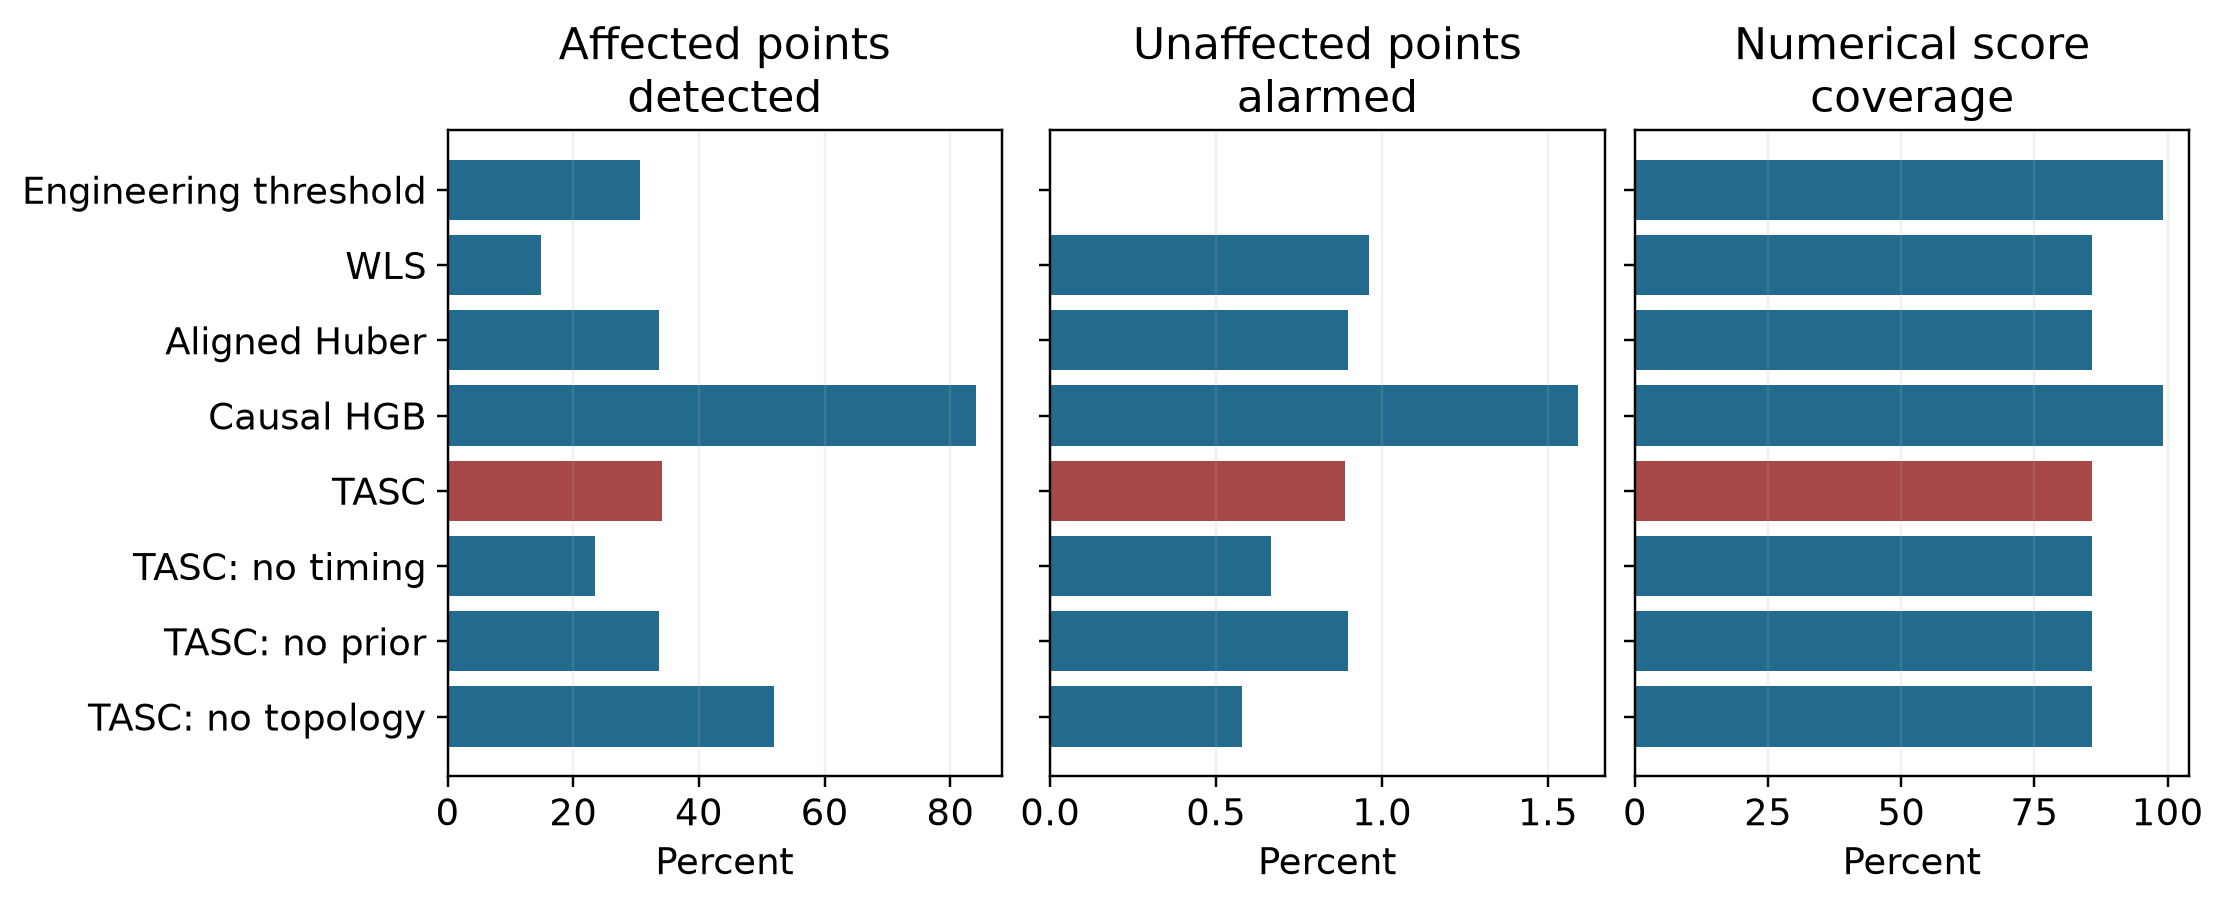
\includegraphics[width=\textwidth]{../shared/comparison.png}
\caption{Detection, false alerts and refusal support are separate outcomes. The combined formulation is not the strongest detector in this matrix.}
\end{figure}

Threshold and forecast leave 16000 entries unscorable; complete-frame projection variants leave 256000. The source-invalid coordinate is excluded in either case, but a constrained method additionally withholds otherwise valid coordinates of that frame. Lower pooled false-positive rate must be interpreted with that support loss. On the common source-valid subset, recall remains 0.341906 for TASC, 0.839938 for prediction and 0.519094 without topology.

\subsection{Paired differences and difficulty response}
The TASC-minus-Huber recall difference is 0.0056875, paired interval $[0.0043750,0.0070938]$. The difference from prediction is $-0.4980312$, interval $[-0.5293133,-0.4610281]$. The difference from no-topology is $-0.1771875$, interval $[-0.1792188,-0.1752812]$. The small gain over aligned Huber is insufficient to support general superiority of the combined formulation.

\begin{figure}[htbp]\centering
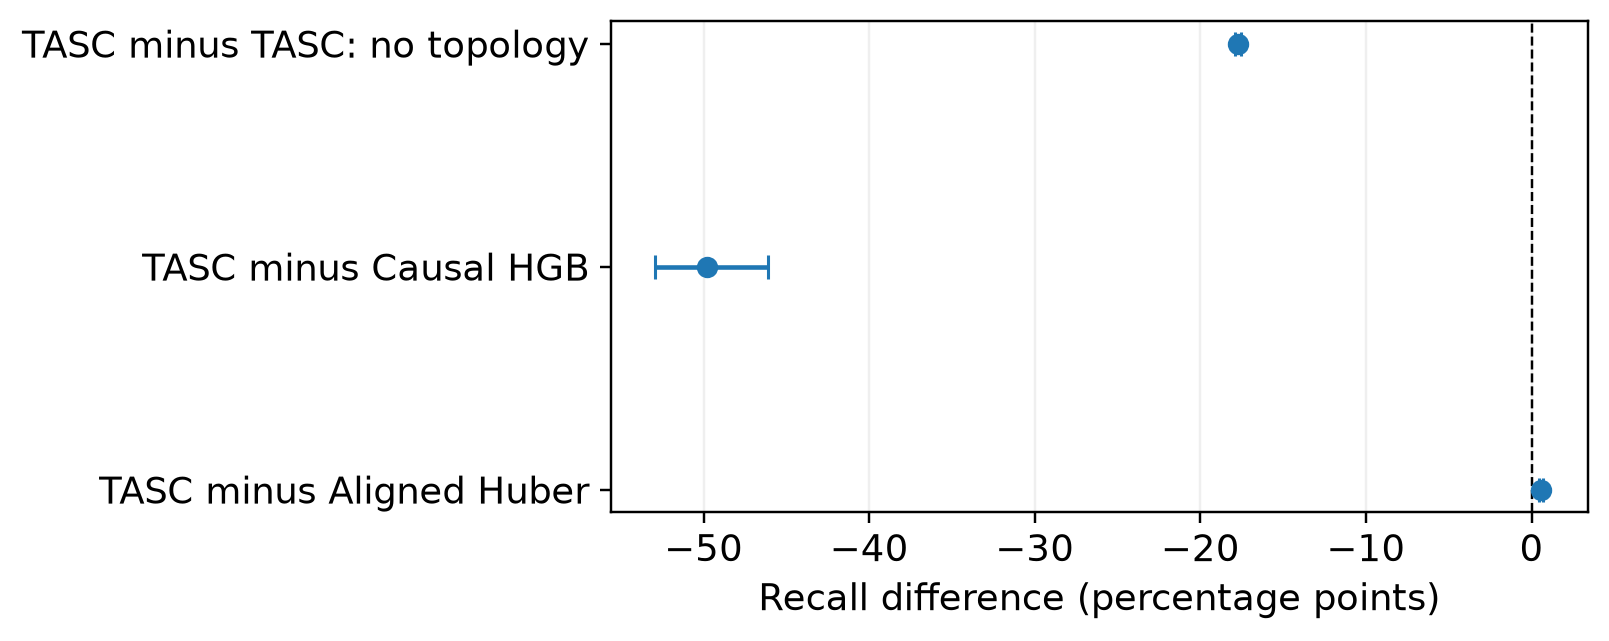
\includegraphics[width=.96\textwidth]{../shared/paired.png}
\caption{Paired recall differences. Repeated protocol slots remain within their seed blocks; they do not artificially multiply independent sample size.}
\end{figure}

\begin{figure}[htbp]\centering
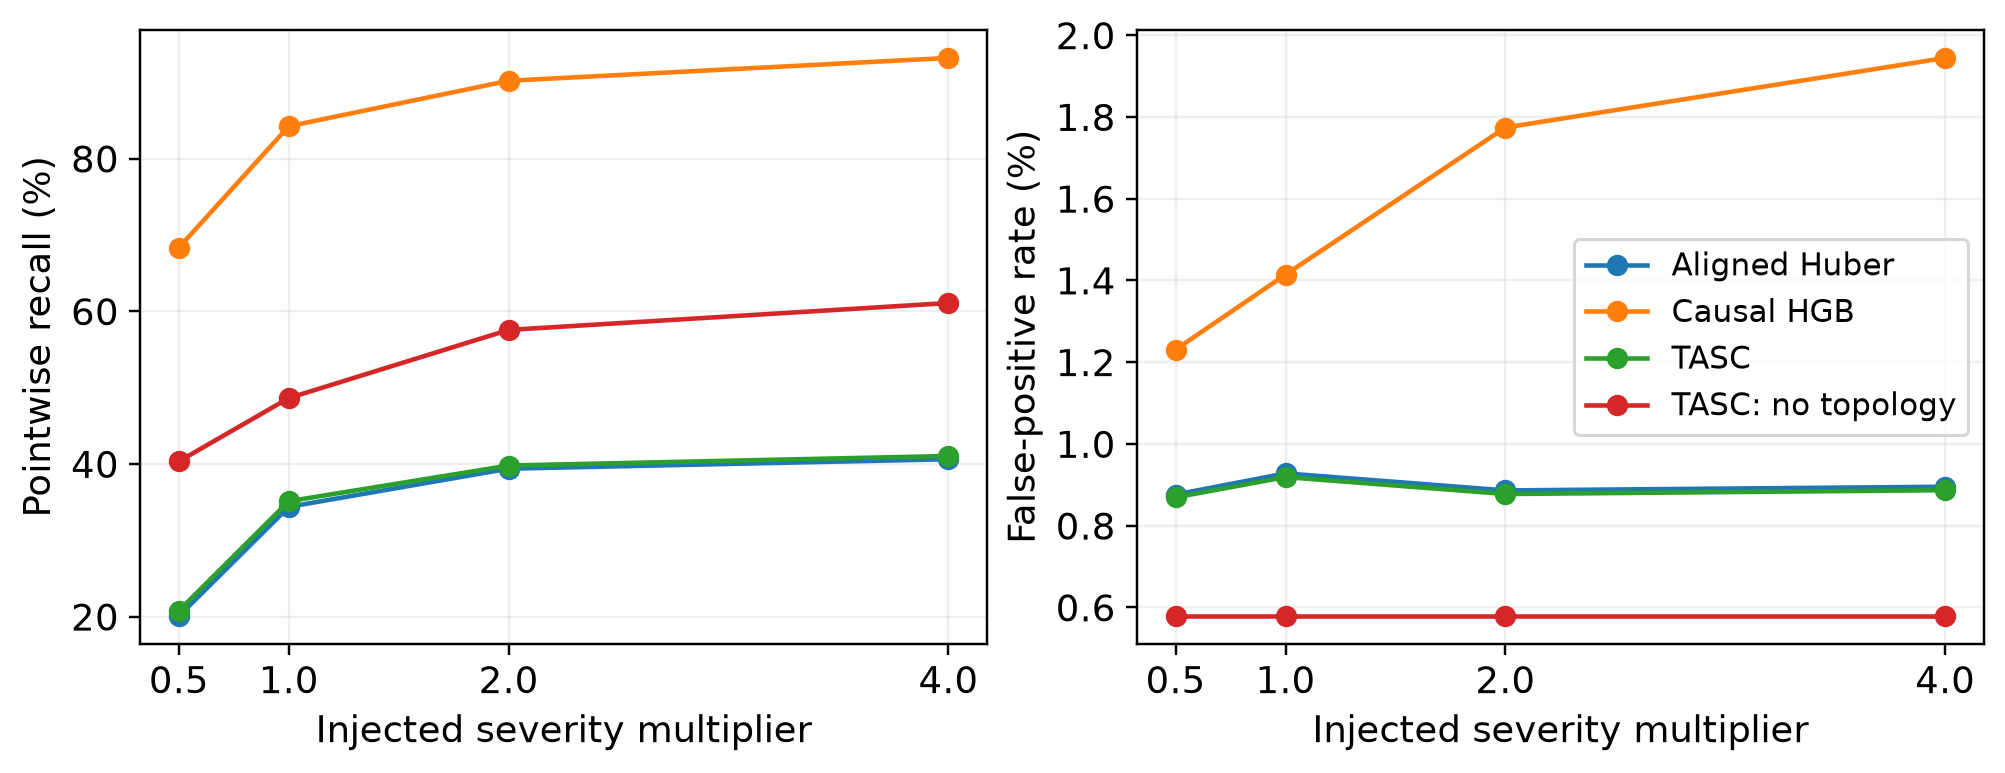
\includegraphics[width=.98\textwidth]{../shared/severity.png}
\caption{Severity response at fixed sensor-noise scale. Magnitude-bearing faults vary while the repeated controls retain their weight.}
\end{figure}

The delay negative control produces 3532 TASC false alerts in the full matrix and has undefined recall because no sensor fault exists. The held-out recovery case with seed 1000 and severity 2 has TASC recall 0.036667 and predictor recall 0.970000. This case combines a changed recovery relation with alignment-boundary effects. These local examples illustrate failure cases; neither is presented as a representative average. A graph-local correction should not be used as proof that the identified instrument failed.

\section{Independent optimization checks}
The production vectorized reweighting is compared with an independently defined Huber objective and gradient. Write $x=y+\operatorname{diag}(\sigma)z$. An SVD null-space parameterization eliminates equality constraints before BFGS, independently of the production iterates. Six families, four availability times and presence/absence of the prior yield 48 systems with fixed numerical seeds.

Maximum absolute objective gap is approximately $2.64\times10^{-12}$, maximum equality residual $6.83\times10^{-13}$ and maximum projected-gradient infinity norm $1.50\times10^{-8}$. Forty-three BFGS runs report success flags and five report non-success flags. All 48 satisfy the stated objective, equality and projected-stationarity criteria. The exported verification retains these flags, but not optimizer status messages. State-coordinate differences alone would also be inappropriate because a Huber problem can have nonunique minimizers.

An independent KKT solution checks the small weighted problem. Aggregate, coverage and event-latency counts are independently reconciled over all 6144 cells. These checks support numerical correctness within the bounded systems. They do not convert the negative localization result into a favorable result or validate the process assumptions.

\section{Discussion and limitations}
\subsection{Why an admissible state is not a diagnosis}
Conservation makes some observation combinations impossible under the model. It does not make the remaining explanation unique. A regularizer derived from upstream feed adds correlated assumed structure, not an independent instrument. When projection distributes a local error over several channels, the correction's spatial explanation can look more specific than the data justify.

The no-topology result is evidence against this particular equality/prior formulation as a stronger detector of the defined disturbances. It does not show that balances should be discarded in operating plants. Mineral-specific constraints, independently measured inventory, process timing and a calibrated error structure may add information absent here. Such changes require a new held-out evaluation rather than tuning the current test matrix until the proposed method wins.

\subsection{External validity and time policy}
The generator is short, seeded and anchored to one operating reference. It omits many nonlinear regimes, chemistry changes, maintenance conditions, correlated errors and industrial modes. Delay metadata are known and normal aligned closure is exact by construction. Quality masks are supplied. The sixteen seeds support descriptive paired comparisons of this authored design, not estimated field reliability.

Real observation semantics introduce a separate limit: source-change time and server confirmation are different~\cite{datavalue}. A constant healthy value can have old source time and current server confirmation. Neither time alone diagnoses a frozen sensing element. The associated interface retains both under an explicit policy and keeps observed quality separate from estimates. The numerical study does not independently validate field quality discovery.

No historian, as-built geometry or production acceptance was available. The fourteen external CAOS examples displayed by the plant interface remain separate source cases; this numerical prior does not dynamically fuse their outputs. No dynamic vessel inventory or validated causal diagnosis is inferred. Operational usefulness needs calibrated site timing, mappings and outcomes beyond these controlled detections.

\section{Reproduction and availability}
The public repository supplies compact observations, masks, current truth, all method scores, full comparison counts, paired analysis and the portable independent optimizer checks. The maintained model functions implement inference; notebooks call them rather than substituting new algorithms. Exact numerical dependencies and disjoint seeds permit reconstruction of the fitted predictor and calibration.

Python 3.12.10, NumPy 2.2.6, SciPy 1.18.1 and scikit-learn 1.9.1 were used with numerical threads bounded to one. Full comparison with the fitted checkpoint took approximately 80.3\,s on the recorded workstation. Raw source cache and checkpoint remain external, with checkpoint digest in the public model manifest. Code, data and computational material: \url{https://github.com/fsantibanezleal/CAOS_OreBridge}.

\section{Conclusion}
Transport alignment and robust constrained optimization can be numerically correct while producing weak discrepancy localization. The combined TASC formulation barely improves aligned-Huber recall and loses to causal prediction and its no-topology ablation on this controlled network. The paired intervals and common-support comparison preserve that result.

A useful interpretation must keep optimization, evidence timing, input quality, coverage and physical identifiability separate. A coherent estimate and a persuasive asset explanation do not establish which instrument or process mechanism caused a discrepancy. Those distinctions remain necessary before extending a plant visualization into operational diagnosis.

\begin{thebibliography}{99}
\small\raggedright
\bibitem{sadeghi} Sadeghi, Hodouin and Bazin (2018). Mineral processing plant data reconciliation including mineral mass balance constraints. \emph{Minerals Engineering}. \url{https://doi.org/10.1016/j.mineng.2018.04.023}.
\bibitem{huber} Huber, P. J. (1964). Robust Estimation of a Location Parameter. \emph{Annals of Mathematical Statistics}, 35, 73--101. \url{https://doi.org/10.1214/aoms/1177703732}.
\bibitem{hgb} scikit-learn. HistGradientBoostingRegressor, maintained documentation, 1.9.1. \url{https://scikit-learn.org/stable/modules/generated/sklearn.ensemble.HistGradientBoostingRegressor.html}.
\bibitem{gdn} Deng, A. and Hooi, B. (2021). Graph Neural Network-Based Anomaly Detection in Multivariate Time Series. \emph{AAAI}. \url{https://arxiv.org/abs/2106.06947}.
\bibitem{gstpro} Zheng, Y. et al. (2024). Graph Spatiotemporal Process for Multivariate Time Series Anomaly Detection with Missing Values. \url{https://arxiv.org/abs/2401.05800}.
\bibitem{datavalue} OPC Foundation. OPC Unified Architecture, Part 4: Services, section 7.11, DataValue. \url{https://reference.opcfoundation.org/specs/OPC-10000-4/7.11}.
\end{thebibliography}

\end{document}
